\documentclass[a4paper,11pt]{article}
\usepackage{fullpage}
\usepackage[latin1]{inputenc}
\usepackage[T1]{fontenc}
\usepackage[normalem]{ulem}
\usepackage[english]{babel}
\usepackage{listings,babel}
\usepackage{palatino}
\usepackage{gensymb}
\lstset{breaklines=true,basicstyle=\ttfamily}
\usepackage{graphicx}
\usepackage{moreverb}
\usepackage{url}
\usepackage{tweaklist}
\renewcommand{\itemhook}{\setlength{\topsep}{0pt}\setlength{\itemsep}{0pt}}
\renewcommand{\enumhook}{\setlength{\topsep}{0pt}\setlength{\itemsep}{0pt}}

\title{TDC core test report}
\author{S\'ebastien Bourdeauducq}
\date{November 2011}
\begin{document}
\setlength{\parindent}{0pt}
\setlength{\parskip}{5pt}
\maketitle{}
\section{The demonstration design}
\subsection{Hardware}

\subsection{Contents}

\subsection{TDC core implementation details}

\begin{figure}[!h]
\centering
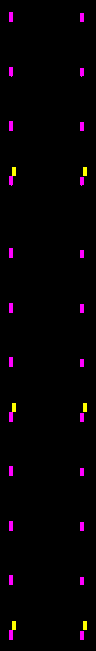
\includegraphics[width=1.6cm]{floorplan.png}
\caption{Floorplan of the delay lines and ring oscillators in FPGA Editor.}
\label{fig:floorplan}
\end{figure}

\begin{figure}[!h]
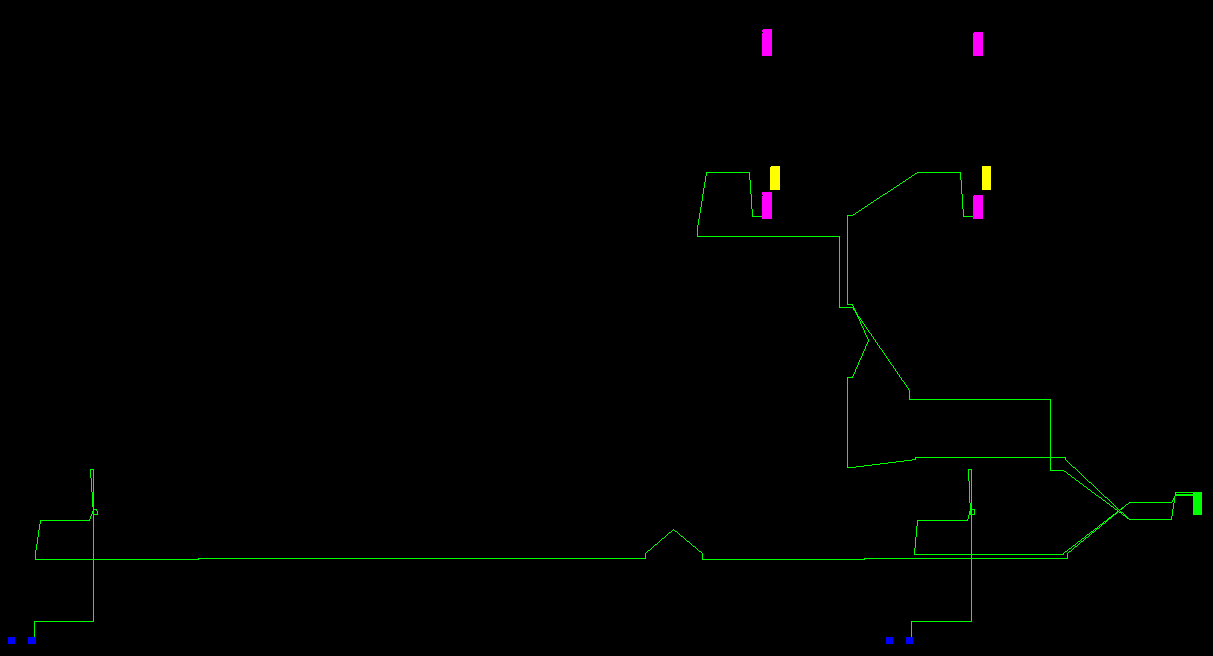
\includegraphics[width=\textwidth]{input_routes.png}
\caption{Input signal path in FPGA Editor.}
\label{fig:inputpath}
\end{figure}

\subsection{Synthesizing and running the design}

\subsection{Command line interface}

\section{Method and results}

\subsection{Temperature measurement with ring oscillators}
\label{sec:rofreq}

\begin{figure}[!h]
\includegraphics[width=\textwidth]{rofreq.pdf}
\caption{Dependence of ring oscillator frequencies on temperature.}
\label{fig:rofreq}
\end{figure}

\subsection{Startup calibration stability}
Temperature is 37C.

\begin{figure}[!h]
\includegraphics[width=\textwidth]{scs.pdf}
\caption{Difference between the LUT contents from two startup calibrations at the same temperature.}
\label{fig:scs}
\end{figure}

\subsection{Differential TDC}

Temperature is 36.9375\degree C
\begin{figure}[!h]
\includegraphics[width=\textwidth]{mhist.pdf}
\caption{Differential measurements}
\label{fig:mhistll}
\end{figure}

\subsection{Temperature compensation}
Even though the influence of temperature is small (\ref{sec:rofreq}), we can still see the action of the online calibration.

We brought the temperature to from 37\degree C to 47.875\degree C, and ran startup calibration again. We observed a significant difference between the LUT contents (figure \ref{fig:chtmlt}).

\begin{figure}[!h]
\includegraphics[width=\textwidth]{chtmlt.pdf}
\caption{Difference between the LUT contents from two startup calibrations at high and low temperatures.}
\label{fig:chtmlt}
\end{figure}

\begin{figure}[!h]
\includegraphics[width=\textwidth]{chtmht.pdf}
\caption{Difference between the LUT contents from startup calibration and the values computed by online calibration.}
\label{fig:chtmht}
\end{figure}

\section{Conclusions}

\end{document}
